\documentclass{beamer}
\title{The Sudoku Project}
\subtitle{WEEK 9: 18/09/2021 to 25/09/2021}
\author[Ishika | Yashvi]{Ishika De and Yashvi Donga}
\date{September 2021}

\usetheme{Madrid}

\begin{document}
\begin{frame}
     \titlepage
\end{frame}
\begin{frame}
     \frametitle{Agenda}
     \begin{itemize}
          \item Brief Overview
          \item Current Status
          \item Toolchain
          \item Learnings
     \end{itemize}
\end{frame}

\begin{frame}
     \frametitle{Brief Overview}
     The goal of this project is to investigate a variety of algorithms (backtracking, brute force, stochastic search and Crook's algorithm) that are capable of solving sudoku puzzles, of ranging difficulties, in order to learn more about sudoku solving techniques.\newline

     We also wanted to use the OpenCV library to read a sudoku from an image and solve it.
\end{frame}

\begin{frame}
     \frametitle{Current Status}   
     \begin{itemize}
		  \item Tested backtracking and brute force algorithm in C++, Java and Python for 100 sudokus of 3 difficulty levels.
		  \item Tested stochastic simulated annealing algorithm and Crook's algorithm in Python - not working for higher difficulty levels.
	 \end{itemize}
\end{frame}

\begin{frame}
     \frametitle{Current Status}   
     \begin{itemize}
		  \item Results
		  \begin{figure}
		  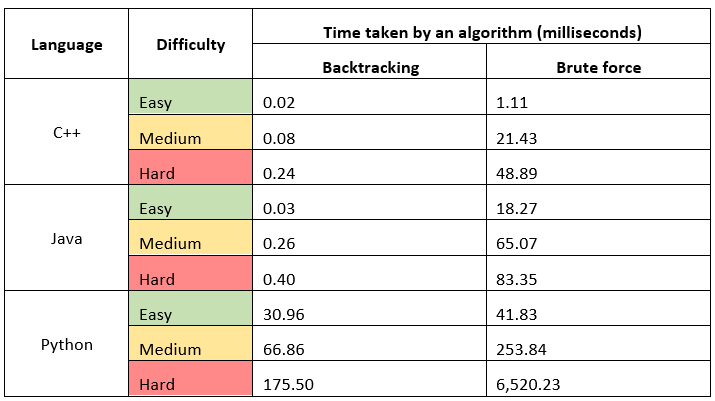
\includegraphics[width=0.9\textwidth]{./week9_img/data.png}
		  \caption{Average time taken to solve a sudoku (tested 100 puzzles).}
		  \centering
		  \end{figure}
	 \end{itemize}
\end{frame}

\begin{frame}
	\frametitle{Current Status}
	\begin{itemize}
	    \item Completed image processing of a sudoku.  
		  \begin{figure}
		  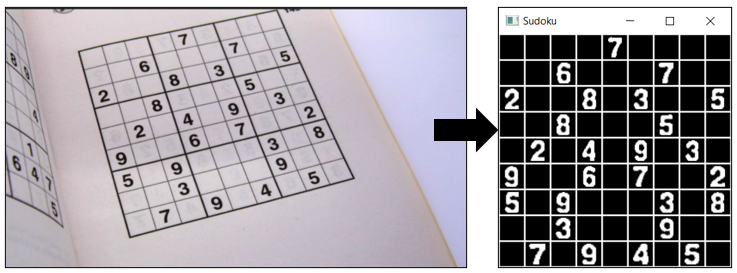
\includegraphics[width=0.9\textwidth]{./week9_img/transformation.png}
		  \caption{Image processing of a sudoku.}
		  \centering
		  \end{figure}
	\end{itemize}
\end{frame}

\begin{frame}
	\frametitle{Current Status}
	\begin{itemize}
		  \item Extracted cells from the sudoku.
			\begin{figure}
			  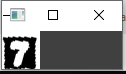
\includegraphics[width=0.4\textwidth]{./week9_img/cell.PNG}
		  \caption{Extracted cell - row 1 and column 5.}
		  \centering
		  \end{figure}
	\end{itemize}
\end{frame}

\begin{frame}
	\frametitle{Current Status}
	\begin{itemize}
		\item Created a CNN model for predicting the digits in the sudoku using MNIST dataset.
		  \begin{figure}
			  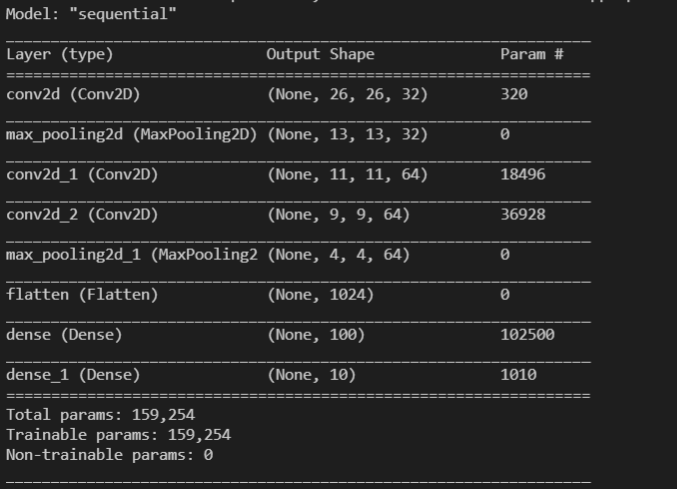
\includegraphics[width=0.6\textwidth]{./week8_img/CNNModel.PNG}
		  \caption{CNN model summary.}
		  \centering
		  \end{figure}
	\end{itemize}
\end{frame}

\begin{frame}
	\frametitle{Current Status}
	\begin{itemize}
		\item Identified the sudoku from the image and solved it using backtracking algorithm.
		  \begin{figure}
			  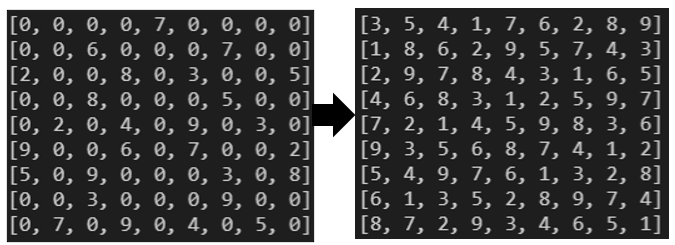
\includegraphics[width=0.8\textwidth]{./week9_img/solve.PNG}
		  \caption{Solved the sudoku from the image}
		  \centering
		  \end{figure}
		  \item Agenda for next week: try to solve sudoku using Haskell and Elixir.
	\end{itemize}
\end{frame}

\begin{frame}
     \frametitle{Toolchain}
     \begin{itemize}
          \item Languages: Python, C++, Java, Haskell, Elixir.
          \item Libaries used in Python: Numpy, OpenCV and Keras.
     \end{itemize}
\end{frame}

\begin{frame}
     \frametitle{Learnings}
	 We learnt to:
     \begin{itemize}
		 \item Collaborate using GitLab.
		 \item Write the same algorithm in different languages.
		 \item Generate data in one language and use the data in another language.
		 \item Explain our code, thought processess and ideas to each other.
		 \item Apply the concept of cost function and thermodynamics in simulated annealing.
		 \item Generate 100 sudokus of 3 different difficulty levels.
		 \item Process an image to extract digits of a sudoku.
		 \item Implement neural networks to predict digits of a sudoku from an image.
	 \end{itemize}
\end{frame}

\end{document}




